\chapter{Einführung in die Ethik der Medizintechnik}

\section{Definition von Ethik und Moral}

Obwohl die meisten von uns wohl ziemlich klare Vorstellungen davon haben, was Moral ist, haben sich die
Philosophinnen und Philosophen bisher auf keine Definition einigen können. Eine ziemlich gute Annäherung:
\begin{quote}
	Wenn wir eine Handlung moralisch beurteilen, dann bringen wir zusätzlich zum eignen Interesse, auch das Wohl und den Wert von anderen Beteiligten ins Spiel (Menschen, als auch Tiere).
\end{quote}
Ethik ist das Teilgebiet der Philosophie, die sich mit der Moral beschäftigt. Ethik ist also eine Theorie oder eine Art, über unser Handeln und uns selbst nachzudenken.

\section{Medizin-/Bioethik}

Die Medizinethik ist eine Teildisziplin der Ethik, die sich mit moralischen Fragen im Gesundheitswesen befasst. Im Englischen ist die \textit{medical ethics} ungefähr gleichbedeutend mit \textit{bioethics}. Im deutschen Sprachraum wird der Ausdruck Bioethik weiter gefasst und bezieht sich auf den Wert, den Anfang und das Ende des Lebens. Die Medizinethik beschäftigt sich mit folgenden Hauptthemen:
\begin{itemize}
	\item Gentechnik (z.B. Klonen)
	\item Präimplantationsdiagnostik, Stammzellenforschung, Schwangerschaftsabbruch
	\item lebenserhaltende Massnahmen, assistierter Suizid, Sterbehilfe, Definition des Todes
	\item körperliche Integrität: Organspenden, \& -handel
	\item Patientenrechte: Informationen, Recht auf Wahrheit; Zwangseinweisungen in Psychiatrie
	\item Verteilungsgerechtigkeit: Medikamente, Spitalbetten, Technologie, Organe
\end{itemize}
Bei den meisten ethisch heiklen Entscheidungen im Gesundheitswesen kommen wir weit, wenn wir vier grundsätzliche Überlegungen berücksichtigen:
\begin{description}
	\item[Selbstbestimmungsrecht (Autonomie) \& Einwilligung der Patienten:] In vielen Fällen gehen wir davon aus, dass Menschen selbst entscheiden können sollen, was mit ihnen geschehen soll. Die Einwilligung des Patienten wird zum dominanten Kriterium für Entscheidungen.
	\item[Würde:] Besteht die Gefahr, dass Menschen als blosses Mittel verwendet werden (z.B. in der medizinischen	Forschung), oder sind sie nicht mehr entscheidungsfähig, so können wir uns auf die Würde eines Menschen	berufen.
	\item[patient’s best interests:] Gewonnene Lebensquantität und -qualität: Wie lange und mit welcher mutmasslichen Lebensqualität (Schmerzen, Behinderungen usw.) wird die	Patientin weiter leben? Was sind die Folgen einer Intervention?
	\item[Gerechtigkeit:] Im Gesundheitswesen geht es zunehmend häufig um die Verteilung von Ressourcen, von denen es nicht genug gibt (Geld, Medikamente, Organe usw.). Hier sollte eine gerechte Verteilung eine zentrale Rolle spielen.
\end{description}
Es ist nicht immer möglich eine Einwilligung vom Patienten zu kriegen. Deshalb überschreiten Ärzte oft die Grenze, wenn sie implizit entscheiden was für den Patienten am besten ist. Eine Einwilligung muss auch gültig sein, sie muss also freiwillig, kompetent und informiert vom Patienten getroffen werden.

\section{Ethik der Medizintechnik}

Über Ethik in der Medizintechnik wird kaum geredet, obwohl man dass eigentlich sollte. Dass liegt wohl daran, dass in der Ingenieursausbildung nicht über Ethik unterrichtet wird. Im englischsprachigen Raum ist Ethik ein Thema in jedem Studiengang. Die Ethik der Medizintechnik befindet sich im Schnittbereich zwischen der Medizinethik und der Ingenieursethik. Ihre Aufgaben ist es Fragen rund um die Forschung, Entwicklung und Herstellung von Medizinprodukten zu diskutieren. Es geht dabei nicht nur um rechtliche Fragen sondern auch um Fragen zum Wohl aller. Die Grundlage für diese Fragen ist in erster Linie die Medizinethik. Dann können auf andere grosse Theorien der Ethik zurückgegriffen werden:
\begin{description}
	\item[Utilitarismus (Nützlichkeit)] kann unter Umständen die Freiheit, Würde oder das Wohl einzelner einschränken
	\item[Menschenwürde (Kant)] ist ein umstrittener Begriff. Die Autonomie eines einzelnen Menschen kann in Kontexten, wo es schwierig ist eine Einigung zu erlangen nicht umgesetzt werden.
	\item[Religiöse Ethik] alles was in der Bibel steht z.B. 10 Gebote (wenn man religiös ist)
\end{description}
Abbildung \ref{fig:entscheidung} zeigt wie man Entscheidungen erklären und bewerten kann.

\begin{figure}
\centering
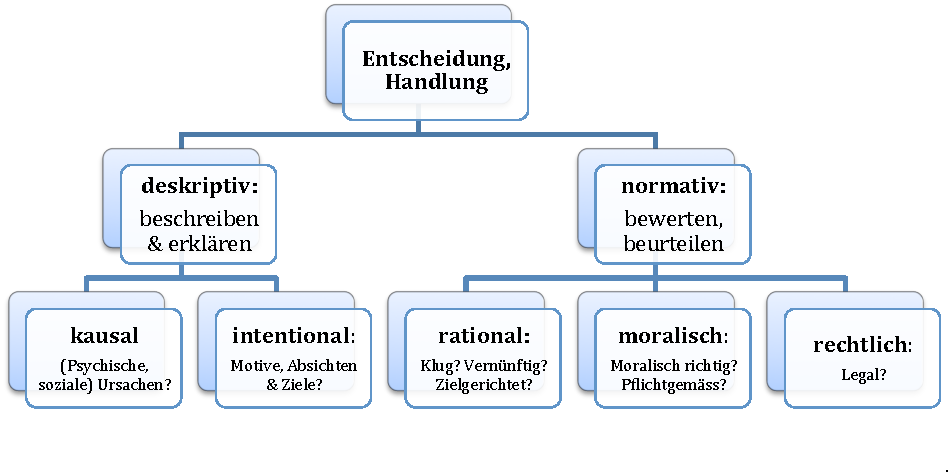
\includegraphics[width=0.7\linewidth]{fig/entscheidung}
\caption{Handlungen erklären \& bewerten}
\label{fig:entscheidung}
\end{figure}
